\section{模板结构}


\par \texttt{WUTthesis}的文件夹中包含以下文件及子文件夹
\begin{itemize}
\item \texttt{Thesis.tex},论文的主源文件;
\item \texttt{WUTthesis.sty},自定义的论文模板宏包;
\item \texttt{Cover.tex},包含封面信息及封面生成命令的源文件;
\item \texttt{Dedications.tex}, 包含“{\kaishu 献给某某某}”字段的源文件;
\item \texttt{Declaration.tex},包含独创性声明和学位论文使用授权书的源文件;
\item \texttt{Abstract.tex},包含中英文摘要的源文件;
\item \texttt{Introduction}等,章文件夹,多个,每一个文件夹对应一章,一章中所涉及的一切子源文件以及插图都包含在相应文件夹中;
\item \texttt{Appendices},附录文件夹,所有的附录源文件都包含在该文件夹中;
\item \texttt{Bibliography.bib},文献数据库文件;
\item \texttt{Achievements.tex},包含作者简历和科研成果的源文件;
\item \texttt{Acknowledgements.tex},包含致谢的源文件;
\item \texttt{STZhongsong.ttf},华文中宋字体文件;
\item \texttt{WUT.jpg},图片形式的“武汉理工大学”。
\end{itemize}
其中,\texttt{Dedications.tex}可有可无,不需要时,只需要将\texttt{Thesis.tex}文件中的对应导入文件的代码删除或注释。另外,该页也以可用其他软件设计生成,随后将生成的\texttt{Dedications.pdf}文档插入即可,对应的操作是将\texttt{Thesis.tex}中的对应代码替换为
\begin{lstlisting}[language=TeX]
\clearpage{\pagestyle{empty}\cleardoublepage} %% 其作用是,如果此页为偶数页,则设为完全空白页,进入下一页
\includepdf{Dedications.pdf} %% 导入Dedications.pdf文档
\end{lstlisting}
即可。关于{\STZhongsong 独创性声明}和{\STZhongsong 学位论文使用授权书}部分,可以打印、签名、扫描后将成生的\texttt{Declaration.pdf}文档插入;对应的操作是将\texttt{Thesis.tex}中的对应导入文件的代码替换为
\begin{lstlisting}[language=TeX]
\clearpage{\pagestyle{empty}\cleardoublepage}
\includepdf{Declaration.pdf}
\end{lstlisting}
即可。每一章的层次结构分为章(chapter)、节(section)、小节(subsection),这里建议每一节的所有内容都写进一个源文件中,然后使用导入命令 \verb"\input{}" 将各个源文件以类似递归的方式链接成一个整体(\texttt{Thesis.tex}中导入对应各章的\texttt{Chapter.tex},各章的\texttt{Chapter.tex}中在导入对应的各节的源文件)。每一章所涉及的所有内容(每一节对应的源文件、图)都存放到一个文件夹,这样做的目的也是为了使整个\texttt{WUTthesis}的结构更加突出,便于用户理解。然而,这样做就面临一个问题,当导入对应节(section)的源文件或图是,都必须提供精准的路径,而当对应每一章的文件夹重命名后,相应章的所有路径都必须改变,这因此会造成一些麻烦。解决的办法是在\texttt{Thesis.tex}中导入每一章源文件前定义一个指代路径的宏 \verb"\path",例如:
\begin{lstlisting}[language=TeX]
\def\path{Introduction}\chapter{引言}\label{chap_introduction}


\section{{\LaTeX}简介}


\begin{WUTquote}{Donald Kunth}
Microsoft Word is the last thing I want to use before I die.
\end{WUTquote}


\par {\LaTeX}是用于产生高品质文档的排版系统,而且事实上已经成为了学术出版的行业标准,国际上绝大多数学术期刊都要求接受{\LaTeX}稿件。{\LaTeX}排版系统基于的是“What you think is what you get.”(所思即所得)的思路\footnote{Microsoft Word、LibreOffice Writer、WPS Writer等排版软件基于的是“What you see is what you get.”(所见即所得)的思路。}。用于只需要关注文档的内容,而计算机会负责相关的格式处理。对于初学者有一定的难度,然而当熟练之后,{\LaTeX}便具有压倒性的优势,尤其是排版大型文档时,比如学位论文或书籍。{\LaTeX}的前身是1978年发布的{\TeX}排版系统,发明人为Donald Kunth教授(图~\ref{fig_Knuth})。1984年,Leslie Lamport博士编写了一组自定义命令宏包,取名LaTeX,该宏包对{\TeX}系统的若干命令进行了重新封装,使得整个排版系统使用起来方便了许多,并于次年发布了LaTeX宏包的源程序。逐渐的,{\TeX}排版系统也就演变为我们今天熟称的{\LaTeX}排版系统。{\LaTeX}是一个开源项目(\url{https://www.latex-project.org/}),世界各地的爱好者为{\LaTeX}系统编写了若干宏包,用于根据用户需求进行各式各样的格式处理,这些宏包及相关的说明文档可以从CTAN网站(Comprehensive {\TeX} Archive Network,\url{https://www.ctan.org/})下载。目前,国际上最大的{\TeX}/{\LaTeX}排版系统的用户组织为TUG(The TeX Users Group,\url{https://www.tug.org/})。关于{\LaTeX}的详细介绍,可以参考相关书籍\cite{Hu_2013, Liu_2013, Knuth_1986, Mittelbach_2004},或是相关的网络资料。



\begin{figure}
\begin{center}
\begin{minipage}[t]{0.7\hsize}
\resizebox{1.0\hsize}{!}{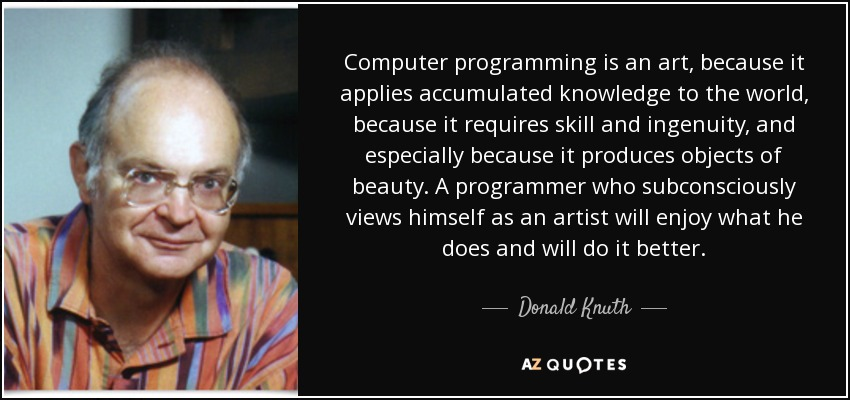
\includegraphics{\path/Knuth.jpg}}
\end{minipage}
\end{center}
\caption{{\TeX}系统的发明人Donald Kunth教授。}
\label{fig_Knuth}
\end{figure}







\section{\texttt{WUTthesis}}



\par 正由于{\LaTeX}在诸多方面的优势,国内越来越多的大学都开始鼓励采用其作为学位论文的排版系统,尤其是对于理工科专业。针对各大学学位论文的格式要求,一些校友们也已经制作了相应的学位论文{\LaTeX}模板。这里值得特别提出的是,在制作并推广学位论文{\LaTeX}模板方面,已经有两位武汉理工大学的校友作出过努力,他们的个人信息、作品名称,作品网址列出如下:
\begin{itemize}
\item 胡卫谊,2010年硕士研究生毕业,武汉理工大学计算机科学与技术学院,
\begin{itemize}
\item 作品:《武汉理工大学学位论文{\LaTeX}模板\texttt{WHUTthesis}》(研究生),
\item 作品网址:\url{https://code.google.com/archive/p/whutthesis/},
\item 作者邮箱:\texttt{whutthesis@gmail.com};
\end{itemize}
\item 曹宇,2015年本科毕业,武汉理工大学交通学院,
\begin{itemize}
\item 作品:《武汉理工本科论文{\LaTeX}模板》,
\item 作品网址:\url{https://github.com/tsaoyu/WHUT-LaTeX-bachelor},
\item 作者邮箱:\texttt{thesis@tsaoyu.com}。
\end{itemize}
\end{itemize}
但可惜的是,到目前位置(2020年2月),他们的工作并没有得到官方的认可,反而在提交学位论文进行反剽窃检查时,被要求提供doc格式的文档\footnote{此处省去太多吐槽。}。胡卫谊制作的模板因为长时间没有维护,再加上该模板在结构等方面存在一些需要改进和提升的地方,所以有必要重新制作新的模板,而本文就是针对这一目的介绍一种新的武汉理工大学研究生学位论文{\LaTeX}模板:\texttt{WUTthesis}。该新模板是根据《武汉理工大学博士、硕士学位论文撰写、印刷格式的统一要求(2009年7月修订)》制作的,模板在制作方面遵循一下原则:
\begin{itemize}
\item 模板要尽可能的简单,不做过多的封装,尽量将一些格式设置放在主文件的导言区。过多的封装会隐藏模板设计细节,从而影响用户对模板的理解。(这里鼓励用户在遵循学校统一格式要求和充分理解设计细节的情况下,根据自己的需求对模板进行修改。)
\item 模板的结构必须和学位论文的结构保持一致,从而可以使用户能快速且直观地理解模板的结构。
\end{itemize}


\par \texttt{WUTthesis}的改进和提升需要官方的配合,以及使用者的不断反馈。广大用户针对\texttt{WUTthesis}如果发现什么问题,或是有什么意见或建议,请联系作者本人,邮箱为\texttt{gujiayin1234@163.com}。{\color{red} 这里必须声明如下:由于\texttt{WUTthesis}格式上无法100\%地保证没有任何问题,再者,因为\texttt{WUTthesis}还未得到官方认可(到2020年2月为止),最终会要求在网上系统提交doc格式的文档,由此可能会引起的潜在种种问题,作者本人概不负责。}




\section{{\LaTeX}安装}

\par 下面列出一些{\LaTeX}套装以及相应的适用操作系统和官方网站
\begin{itemize}
\item MiKTeX (Microsoft Windows, \url{https://miktex.org/});
\item MacTeX (macOS, \url{https://www.tug.org/mactex/});
\item CTeX (Microsoft Windows, Chinese TeX, \url{http://www.ctex.org/HomePage})\footnote{这里需要区分CTeX套装和{\CTeX}宏集。};
\item TeX Live (Unix-like/Microsoft Windows/macOS, \url{http://tug.org/texlive/})。
\end{itemize}
如果在Ububtu(Linux的一种发行版)操作系统下,可以直接通过命令\texttt{sudo apt-get install texlive-full}安装。因为TeX Live具有最广泛的操作系统适用性,所以也自然成为最为推荐的{\LaTeX}套装,其相应的编辑器为 \href{http://www.tug.org/texworks/}{TeXworks}(Linux系统下需要单独安装并通过配置指定已安装的Tex Live可执行文件路径。)\footnote{TeXworks是一种开源的、跨平台、多语言支持的TeX/LaTeX编辑器。其他类似的编辑器包括 \href{https://www.texstudio.org/}{TeXstudio}、\href{https://www.xm1math.net/texmaker/}{Texmaker} 等。}。另外,需要指出的是,CTeX套装虽然针对中排版的{\LaTeX}系统,由于以下两个原因:
\begin{itemize}
\item 截止到2020年2月的最新版本,CTeX套装中并没有包含\texttt{biblatex-gb7714-2015}宏包(该宏包用于设置中文参考文献样式);
\item 其配套的WinEdt\footnote{\href{http://www.winedt.com/}{WinEdt} 是闭源软件,只适用与Microsoft Windows平台,不过用户可以免费使用该软件。}编辑器中并没有发现对应于\texttt{biblatex}宏包的参考文献处理程序\texttt{biber}按钮;
\end{itemize}
不建议使用。而实际上,由于上述原因,\texttt{WUTthesis}也未在CTeX套装上测试成功。不过新版CTeX套装预计会在2020年4月之前发布,变动会很大,我们拭目以待。当然,这里也鼓励喜欢钻研{\LaTeX}技术用户尝试解决上述两个原因造成的在使用\texttt{WUTthesis}过程出现的问题。


















\end{lstlisting}
之后每当我们导入源文件或图时,提供 \verb"\path" 作为路径即可,重命名每一章文件夹时,只要更改对应路径的宏定义就行。通过一些设置,编译生成pdf文档中每一章的开启都位于奇数页,且开启页隐藏页眉也页码,相应的,结束页的页码为偶数,如果此时恰好结束页空白,则该页将隐藏页眉和页码。关于页码,从摘要到第一章开始前,使用罗马数字,而从第一章开始,重新编号,使用阿拉伯数字。在\texttt{Thesis.tex}中关于目录的代码如下:
\begin{lstlisting}[language=TeX]
\begin{spacing}{1.3}
\tableofcontents
\end{spacing}
\end{lstlisting}
这里的\texttt{spacing}环境由\texttt{setspace}宏包提供,其参数用于控制行距(在参数$1.3$的情况下,使用\texttt{spacing}环境和不使用\texttt{spacing}环境,排版效果是一样的)。用户可以根据实际情况,适当调整目录的行距,使得目录尽量控制在两页之内。这里需要说明一下,由于汉字都是方块字,这和英文具有大小写的情况不同,所以使用{\CTeX}宏集提供的\texttt{ctexbook}文类时,行距会自动调整为英文情形下的$1.3$倍。\texttt{Thesis.tex}中对于文献打印部分的代码
\begin{lstlisting}[language=TeX]
\begin{spacing}{1.3}
\printbibliography[heading=bibintoc, title={参考文献}]
\end{spacing}
\end{lstlisting}
是同样的道理,用户可以根据实际情况,调整参考文献的行距。{\color{red}关于书脊部分信息,可以在打印论文封面时让打印店老板操作一下,一般情况下他们都会知道怎么做。}


